%% LyX 2.3.0rc2 created this file.  For more info, see http://www.lyx.org/.
%% Do not edit unless you really know what you are doing.
\documentclass[12pt,english]{scrartcl}
\usepackage[T1]{fontenc}
\usepackage[latin9]{inputenc}
\usepackage{color}
\usepackage{babel}
\usepackage{array}
\usepackage{longtable}
\usepackage{booktabs}
\usepackage{url}
\usepackage[unicode=true,
    pdfusetitle,
    bookmarks=true,
    bookmarksnumbered=false,
    bookmarksopen=false,
    breaklinks=true,
    pdfborder={0, 0, 0},
    pdfborderstyle={},
    backref=false,
    colorlinks=true,
    linkcolor=blue,
    urlcolor=blue]
    {hyperref}
\usepackage{pdfpages}

\makeatletter

%%%%%%%%%%%%%%%%%%%%%%%%%%%%%% LyX specific LaTeX commands.
%% Because html converters don't know tabularnewline
\providecommand{\tabularnewline}{\\}

\makeatother

\begin{document}

\title{Syllabus for General Entomology AL/BI 345 - Fanuchanan 2021}

\author{Aubrey Moore}

\maketitle

\newpage
\tableofcontents

\newpage
\section{Place and Time}

Labs and lectures will take place in ALS 124, which is the teaching
lab in the Agriculture and Life Sciences Building.
\begin{itemize}
\item Lectures: Mondays and Wednesdays, 12:45 - 2:05
\item Labs: Wednesdays 2:20 - 5:15
\end{itemize}

\section{Instructor and Contact Information}

Dr. Aubrey Moore
\begin{itemize}
\item Cell phone: 686-5664 (Please feel free to call at any time.)
\item Office: 735-2086
\item Email: aubreymoore@triton.uog.edu
\item Office: 105H ALS
\item Office hours: by appointment
\end{itemize}

\section{Course Description (from the UoG Catalog)}

This course is an overview of insect biology with emphasis on fundamental
problems encountered by insects, and the structural and functional
adaptations used to overcome these problems. The laboratory focuses
on insect identification. An insect collection is required. The course
meets for three hours of lecture weekly. Prerequisites: BI157-157L
or AL109 or AL281. 

\section{Required Text Book}

Borror, D. J. and R. E. White 1970. \href{https://www.amazon.com/Field-Guide-Insects-America-Mexico/dp/0395911702}{A Field Guide to Insects}.
Houghton Mifflin ISBN 0-395-91170-2.

\newpage
\section{Curricular Mapping}

\subsection{Institutional Learning Objectives (from the UoG Catalog)}

Some of the expected fundamental knowledge, skills, and values that
the University of Guam student will have demonstrated upon completion
of any degree are:
\begin{enumerate}
\item Mastery of critical thinking and problem solving
\item Mastery of quantitative analysis
\item Effective oral and written communication
\item Understanding and appreciation of culturally diverse people, ideas,
and values in a democratic context
\item Responsible use of knowledge, natural resources, and technology
\item An appreciation of the arts and sciences
\item An interest in personal development and lifelong learning
\end{enumerate}

\subsection{Program Learning Objectives (from the UoG Catalog)}

\subsubsection{Learning Objectives for Agriculture Students}

Disciplinary Knowledge: Graduates apply their agricultural knowledge
and skills in the production of agricultural products using best management
practices and addressing locally important issues such as island pocket
economies, conservation, invasive species and endangered species problems.
They use their knowledge and understanding of scientific concepts
to diagnose and solve problems in agricultural fields.
\begin{enumerate}
\item Quantitative Skills: Graduates apply numerical methods in research
design, financial analysis, pesticide and fertilizer application,
irrigation and field setup and use computers for analysis of data
and preparation of reports of results.
\item Research/laboratory skills: Graduates are competent in basic laboratory
procedures and safety in the laboratory and the field. Students will
develop applied thinking skills to help them formulate testable hypotheses
and create effective experimental designs.
\item Communication Skills: Graduates can gather and assess evidence and
use it to create effective lab and scientific reports, and oral presentations.
They will develop the ability to identify, summarize and effectively
communicate current issues to given audiences.
\item Technological Literacy: Graduates are competent at applying technological
skills to their chosen work. They are also competent in the use of
analog and digital equipment used in modern agricultural systems.
Graduates effectively judge the usefulness and appropriateness of
existing and new technologies in their professional endeavors.
\item Professionalism: Graduates work effectively together in teams in laboratory,
community and field settings while following ethical principles in
analysis and communication. Graduates apply their gained knowledge
in addressing natural resource and social issues.
\end{enumerate}

\subsubsection{Learning Objectives for Biology Students}

Disciplinary knowledge and skills: Graduates use their knowledge and
understanding of essential concepts to solve problems in ecology,
genetics, molecular biology, systematics, and evolution. They can
apply their biology knowledge and skills to locally important issues
such as island biogeography, conservation, and endangered species
problems. They apply relevant concepts from chemistry and physics
to biology problems.
\begin{enumerate}
\item Quantitative skills: Graduates apply numerical methods in research
design, and use computers for analysis manipulating and modeling biological
data.
\item Research/laboratory skills: Graduates are competent in basic biology
procedures and safety in the laboratory and the field; they formulate
testable hypotheses and create effective experimental designs using
their knowledge, understanding, and practical experience of scientific
instruments.
\item Communication skills: Graduates use scientific literature and diagrams
as a source of information, properly cite sources and avoid plagiarism,
and create text and graphics to communicate results effectively through
print and oral presentations. They collect and assess evidence and
use it to create effective arguments in writing scientific reports
and proposals.
\item Digital Literacy: Graduates use and process information in multiple
formats via computer. Graduates are competent in the following computer
skills as related to their science work: desktop competencies, word
processing, presentation, and data retrieval and manipulation. Graduates
effectively judge the usefulness and accuracy of external sources
of information.
\item Professionalism: Graduates work effectively together in teams in a
laboratory and field settings and follow ethical principles underlying
scientific research and publication. Graduates understand and apply
the values and limitations of scientific research in addressing public
policy issues.
\end{enumerate}

\subsection{Student Learning Outcomes for AL/BI 345}

Upon completion of AL/BI 345, General Entomology:
\begin{enumerate}
\item Students will be able to accurately identify any insect on Guam to
the taxonomic level of Order and in most cases to Family.
\item Students will be familiar with the behavior and biology of common
insects on Guam.
\item Students will know how to collect insects and preserve them as museum
quality specimens with proper labeling.
\item Students will have an understanding of the importance of insects in
ecosystem function.
\item Students will be aware of negative impacts of invasive species on
Guam's ecosystems and economy.
\item Students will know how to find detailed information on insects in
online resources and in the scientific literature.
\end{enumerate}

\section{Schedule}

A schedule of classes and examinations is available on the home page of the course web site at \url{https://aubreymoore.github.io/ALBI-345}.

\section{Grading}

\begin{longtable}{llc}
\toprule 
Activity                             & Date/Deadline & Maximum Points\tabularnewline
\midrule
Exam 1                               & September 15  & 15\tabularnewline
Exam 2                               & October 27    & 15\tabularnewline
Exam 3                               & December 6    & 15\tabularnewline
\midrule
Insect Collection                    & November 24   & 35\tabularnewline
Research Project - written report    & December 1    & 10\tabularnewline
Research Project - oral presentation & December 1    & 10\tabularnewline
\midrule 
Total                                &               & 100\tabularnewline
\bottomrule
\end{longtable}

\newpage

Final grades will be awarded according to this table.
\begin{longtable}{cc}
\toprule
Total Points & Grade\\
\midrule
90 - 100 & A\\
80 - 89 & B\\
70 - 79 & C\\
60 - 69 & D\\
0 - 59 & F\\
\bottomrule
\end{longtable}

\section{Course Guidelines}

\subsection{Course Web Site}

This syllabus, all handouts and other course resources are available
from the course web site at \url{https://aubreymoore.github.io/ALBI-345}.

\subsection{Examinations}
\begin{itemize}
\item Examinations are cumulative, meaning that you may be asked questions
on any topics covered between the start of the course and the date
of the exam.
\item All exams are 'open book' and you are free to use digital devices
and online resources.
\item Part of each exam will be spent identifying insect specimens. 
\end{itemize}

\subsection{Research Project}
\begin{itemize}
\item Research projects will be done by teams of 1, 2 or 3 people.
\item Each team will make an oral presentation to propose their project
during the October 10 lab period.
\item Each team will submit a written research report and make an oral presentation
during the November 20 lab period.
\end{itemize}

\subsection{Insect Collection}
\begin{itemize}
\item You will be required to collect and preserve at least 35 different insect species
from at least ten taxonomic orders. 
\item Immature insects and soft bodied specimens requiring preservation in alcohol will not be accepted.
\item We will use an iNaturalist project,  \url{https://www.inaturalist.org/projects/insects-of-micronesia}, 
to record data for each specimen in the collection. I will provide
software to print a catalog and pin labels using data stored in the iNaturalist database.
\item Lepidoptera must have their wings spread.
\item Your collection must contain two or more smaller species mounted on paper points.
\item Each specimen must be identified at leased to taxonomic order and labeled properly. 
\item You will receive a maximum of 35 points for your collection. You will
get one point for each specimen which:

\begin{itemize}
\item is properly preserved (moths and butterflies spread; insects too small
to pin on paper points) 
\item has an observation record in iNaturalist
\item is properly labeled
\end{itemize}
\item Points will not be given for duplicate specimens from the same species
\item You are encouraged to collect more than 35 specimens to so that you have 35 specimens which qualify for points.
\end{itemize}

\section{UOG Disabilities Policy}

In accordance with the Americans with Disabilities Act (ADA) of 1990 and the Rehabilitation Act of 1973, the University of Guam does not discriminate against students and applicants on the basis of disability in the administration of its educational and other programs. The University offers reasonable accommodations for a student or applicant who is otherwise qualified, if the accommodation is reasonable, effective and will not alter a fundamental aspect of the University's program nor will otherwise impose an undue hardship on the University, and/or there are not equivalent alternatives. Students are expected to make timely requests for accommodation, using the procedure below.

\subsection{ADA Accommodation Services}

If you are a student with a disability who will require an accommodation(s) to participate in this course, please contact the Student Counseling and Advising Service Disability Support Services office to discuss your specific accommodation needs confidentially. A Faculty Notification letter will be emailed to me specifying your approved accommodations. If you are not registered, you should do so immediately at the Student Center, Rotunda office \#5, \href{mailto:sssablan@triton.uog.edu}{sssablan@triton.uog.edu} or ph/TTY: 735-2460, to coordinate your accommodation request.

\appendix

%\section{Schedule for AL/BI 345 General Entomology Fanuchanan (Fall) 2021}
%\label{schedule}
%Please see next page.
%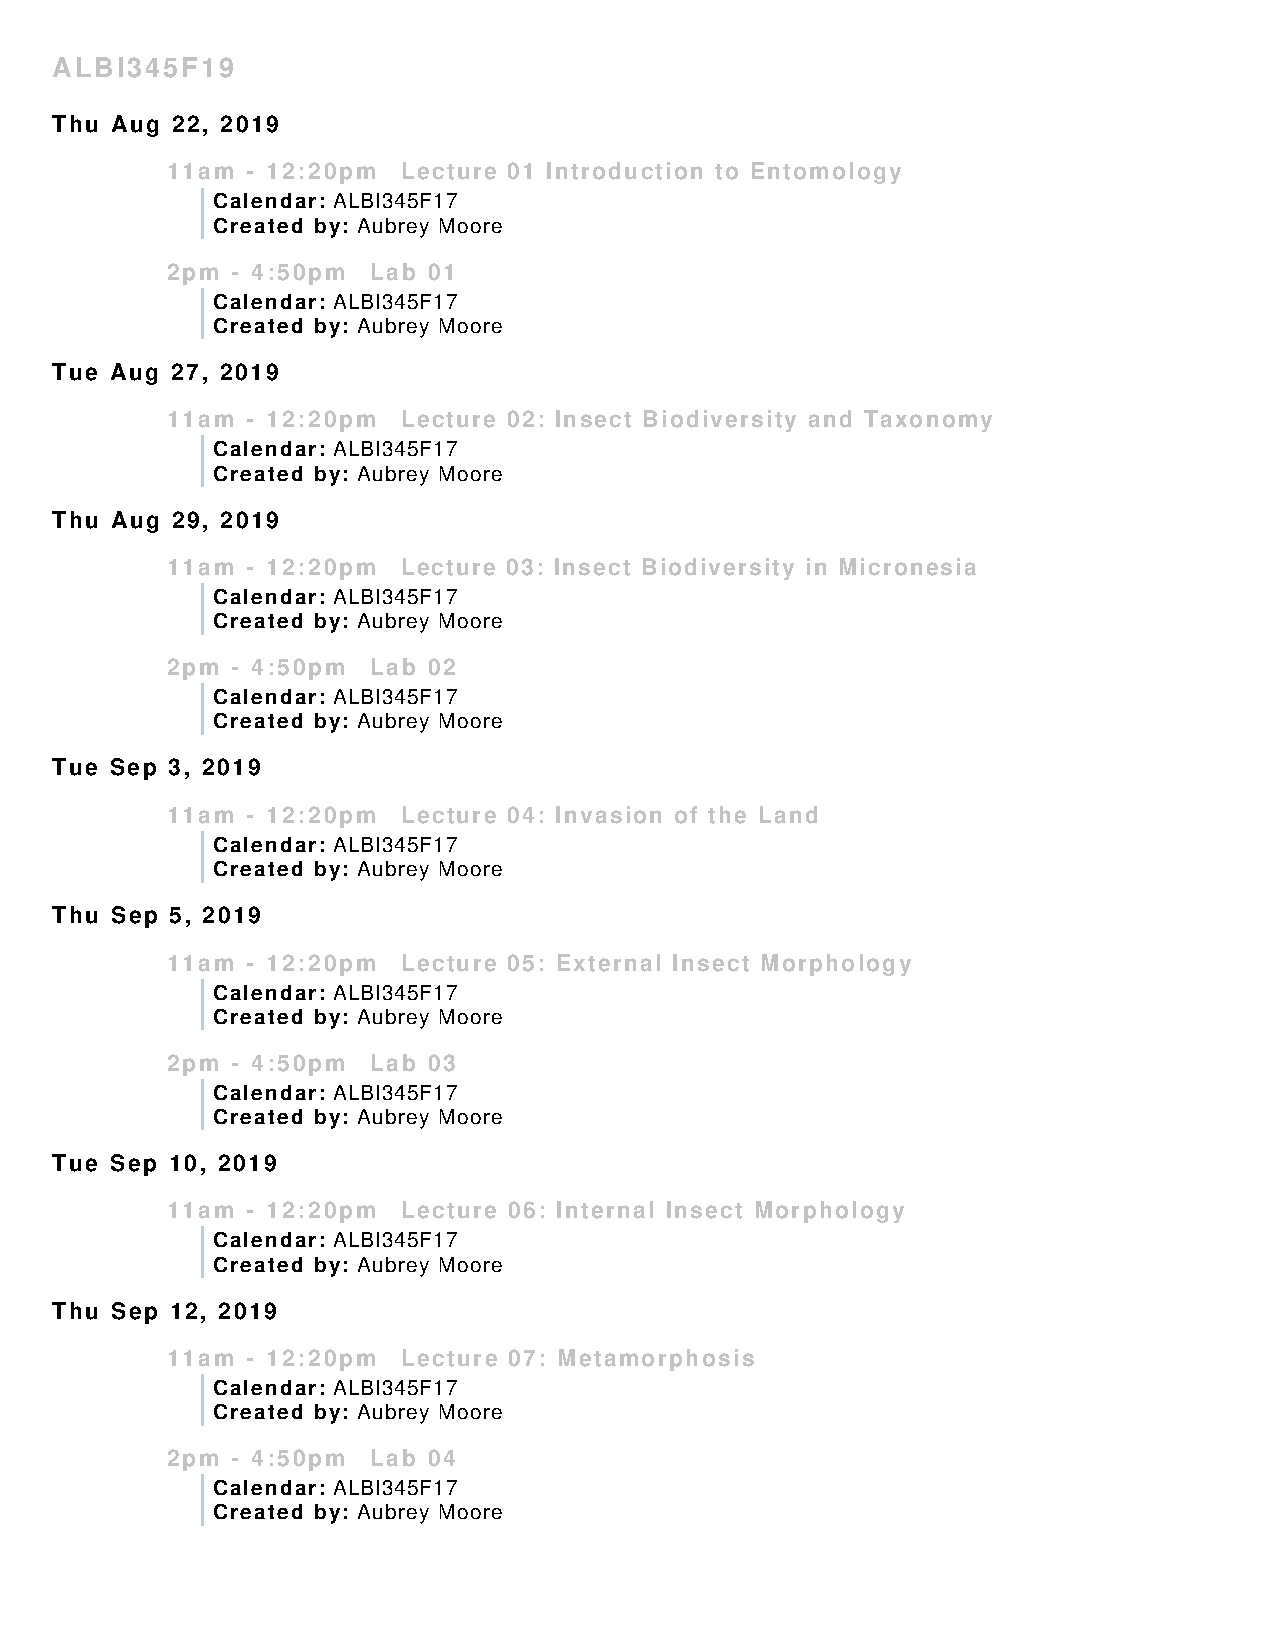
\includepdf[pages=-]{agenda.pdf}

\end{document}
